\documentclass[10pt,handout]{beamer}
% Preamble (fold)

\usepackage[utf8x]{inputenc}
\usepackage{amsmath}
\usepackage{amsthm}
\usepackage{amssymb}
\usepackage[english]{babel}
\usepackage{hyperref}
\usepackage{esint}

\def \postcode {??}
\def \city {Uppsala}
\def \englishinst {Department of Mathematics}
\def \englishuniversity {Uppsala University}
\def \englishtitle {Neural networks and PDE}

\newcommand{\englishindent}{\setlength\parindent{18pt}\setlength\parskip{0pt}}


\providecommand{\e}{\varepsilon}
\newcommand{\R}{\mathbb{R}}
\newcommand{\N}{\mathbb{N}}
\renewcommand{\phi}{\varphi}

\DeclareMathOperator{\esssup}{ess\,sup\ }
\DeclareMathOperator{\essinf}{ess\,inf\ }
%\renewcommand{\sup}{\textrm{sup }}
%\renewcommand{\inf}{\textrm{inf }}
\renewcommand{\div}{\textrm{Div }}
\providecommand{\transpose}[1]{#1^{\intercal}}
\providecommand{\D}[2]{\frac{\partial #1}{\partial #2}}
\providecommand{\norm}[1]{\left\lVert#1\right\rVert}
\providecommand{\supp}{\textrm{supp}}
\providecommand{\sint}{-\!\!\!\!\!\!\int}
\providecommand{\siint}{\text{---}\!\!\!\!\!\!\!\!\iint}
\providecommand{\rquad}{\!\!\!\!\!\!}


% for themes, etc.
\mode<presentation>
\usetheme{Boadilla}
\usecolortheme{seagull}
{ \usetheme{boxes} }

\usepackage{times}  % fonts are up to you
\usepackage{graphicx}
\usepackage{bm}
%\setbeamercovered{transparent}
\newtheorem{Conjecture}{Conjecture}
\newtheorem{question}{Question}
\providecommand{\Ehyp}{E^{hyp}}

\begin{document}

% these will be used later in the title page
\title{\englishtitle}
\author[Avelin]{Benny Avelin \\
	(J. Work with K. Nyström)}
\date[Uppsala-Tokyo Tech] % (optional)
{The 6th Uppsala University - Tokyo Tech Joint Symposium}
% Preamble (end)

\begin{frame} % Title page
\titlepage
% \begin{center}
% 	\includegraphics[scale=0.5]{Images/umu.pdf}
% \end{center}
\end{frame}

\begin{frame} % Outline of my Talk
	\frametitle{Outline}
	\begin{enumerate}
		\item Motivation
		\item Connection to PDE
		\item Some results
	\end{enumerate}
\end{frame}

\begin{frame}
	\frametitle{Motivation (What is machine learning)}
	Three types of problems
	\begin{itemize}
		\item Supervised Learning
		\begin{itemize}
			\item Learning with a teacher
			\item {\bf Ex: }Regression / Classification
		\end{itemize}
		\pause
		\item Unsupervised Learning
		\begin{itemize}
			\item Learning representations
			\item {\bf Ex: }Density estimation, dimensionality reduction, etc.
		\end{itemize}
		\item Reinforcement Learning
		\begin{itemize}
			\item Learning with a critic
			\item {\bf Ex: }Optimal control
		\end{itemize}
	\end{itemize}
\end{frame}
\begin{frame}
	\frametitle{Supervised Learning}
	\begin{itemize}
		\item Classification
		\begin{itemize}
			\item Image classification: $x$-image, $y$-class. Could be object identification like saying `this is the image of a cat'.
			\item Text classification: Given a snippet of text, what is its subject?
		\end{itemize}
		\pause
		\item Regression
		\begin{itemize}
			\item What is the weight of a person given the height? $x$-height, $y$-length.
			\item Object location: Given that you have an image with a ball in it, where in the image is the ball.
		\end{itemize}
	\end{itemize}
\end{frame}

\begin{frame}{Risk and Hypothesis}
	\begin{itemize}
		\item Let us consider data $(x,y) \sim \mu$, where $x \in \mathbb{R}^n$ and $y \in \mathbb{R}^m$.
		\item A hypothesis is a function $h: \mathbb{R}^n \to \mathbb{R}^m$,
		\item A loss-function $L:\mathbb{R}^m \times \mathbb{R}^m \to \mathbb{R}_+$,
		$$R(h) = \mathbb{E}_{\mu}\left[L(h(x),y)\right], \quad \textbf{Risk}$$
		\item Given a data-set $D = \{(x_1,y_1), \ldots (x_N,y_N)\}$ which are sampled i.i.d. from $\mu$ we also define,
 	    $$R_{emp,D} (h) = \frac{1}{N}\sum_{i=1}^N \left[L(h(x_i),y_i)\right], \quad \textbf{Empirical Risk}$$
		\item Call a set of hypothesis $\mathcal{H}$, the hypothesis space.
		\item test
	\end{itemize}
\end{frame}

\begin{frame}{Risk and Hypothesis}
	\begin{itemize}
		\item Find $h^\ast \in \mathcal{H}$ such that,
		$$R(h^\ast) = \min_{\mathcal{H}} R(h), \quad \textbf{Risk minimization}$$

		\item We dont have access to $\mu$ but we have access to a given data-set $D$, we could try to find $h_D^\ast \in \mathcal{H}$ such that,
		$$R_{emp,D}(h_D^\ast) = \min_{\mathcal{H}} R_{emp,D}(h)$$

		\item We cannot find $h_D^\ast$ in general. Instead we try to find $h \in \mathcal{H}$ such that $R_{emp,D}(h)$ is as small as possible,
		$$R_{emp,D}(h_D^\ast) \leq R_{emp,D}(h), \quad \textbf{Empirical Risk Min}$$
	\end{itemize}
\end{frame}

\begin{frame}{Simple example}
	\begin{center}
		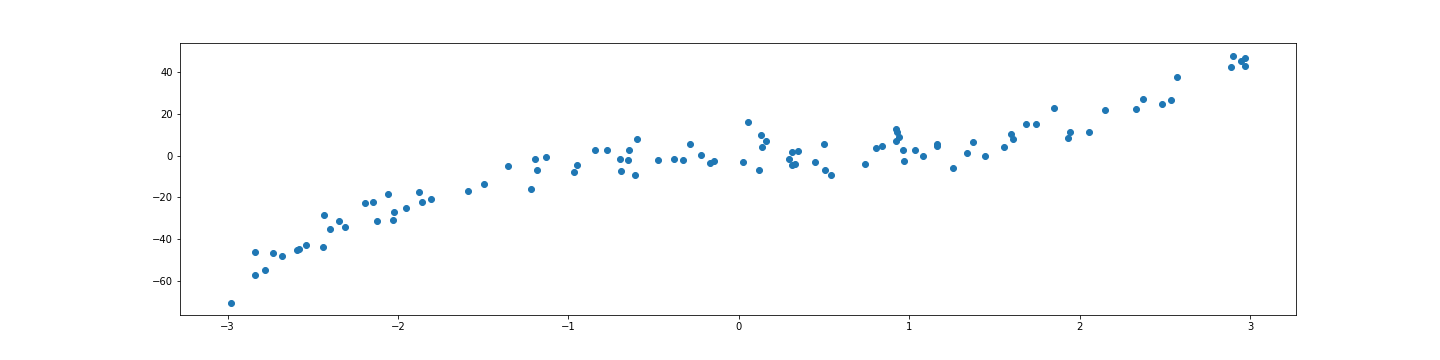
\includegraphics[height=0.3\textheight]{Plots/Regression.png}
	\end{center}
	\begin{itemize}
		\item Let $\mathcal{H}$ be functions of the form
		$$h(x) = \sum_{i=1}^M v_i \sigma (w_i \cdot x + b_i)$$
		for paramters $v_i,w_i,b_i$. $\sigma(x) = \frac{1}{1+e^{-x}}$
		\item Let the loss function be quadratic $L(x,y) = (x-y)^2$
		\item Goal: find $h^\ast_D$ that minimizes
		$$
			R_{emp,D} (h) = \frac{1}{N}\sum_{i=1}^N (h(x_i)-y_i)^2
		$$
	\end{itemize}
\end{frame}
\begin{frame}{Simple Example (Neural networks)}
	\begin{center}
		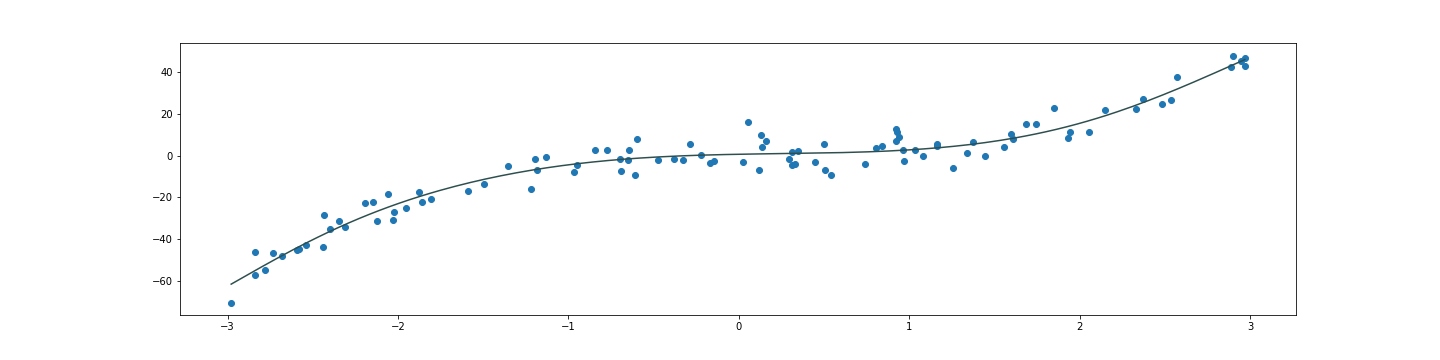
\includegraphics[height=0.3\textheight]{Plots/RegressionFitted.png}
	\end{center}
	\begin{itemize}
		\item $h(x)$ is actually a `single hidden layer neural network'
	\end{itemize}
	\pause
	\begin{center}
		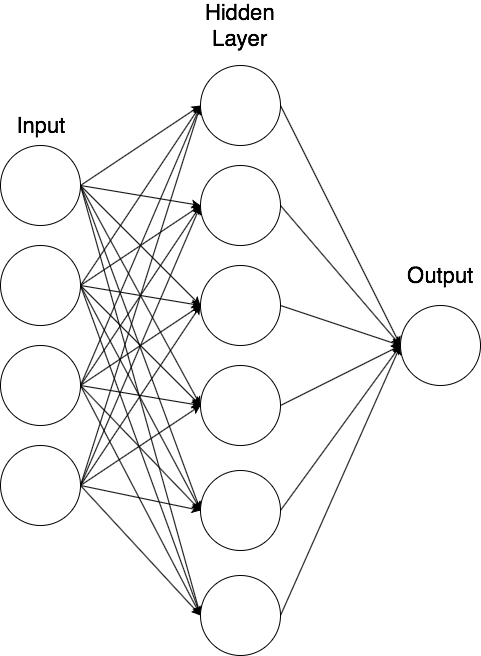
\includegraphics[height=0.25\textwidth]{Images/SingleHidden.png}
		\hspace{1cm}
		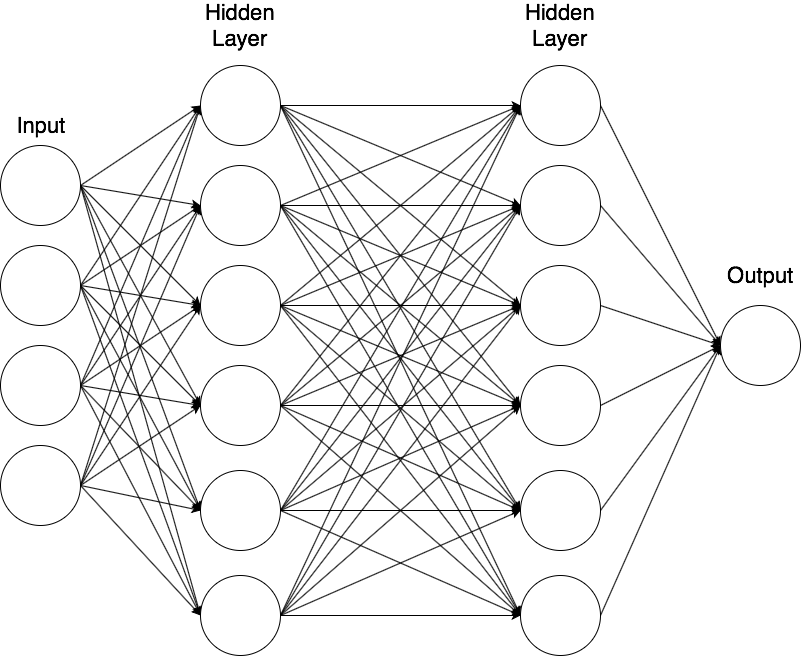
\includegraphics[height=0.25\textwidth]{Images/ManyHidden.png}
	\end{center}
	\pause
	$$h(x) = \sigma \big (W^2 (\sigma (W^1 x + B^1))+B^2 \big )$$
\end{frame}

\begin{frame}{How do we minimize risk?}
	We run a discrete form of gradient flow on the space of weights
	$$
		dW_t = -\nabla_W R_{emp,D}(h_{W_t})dt
	$$
	\begin{itemize}
		\item $W$ is usually very high dimensional 1M and up for many problems
		\item the size of $D$ is also quite big.
		\item run the following discrete process instead
	\end{itemize}
	$$
		\Delta W_i = -\nabla_W R_{emp,D_i}(h_{W_i})\Delta n
	$$
	\begin{itemize}
		\item $D_i$ is a subsampled set of $D$ at each time step $i$, $\Delta n$ is step-length. 
		\item Called Stochastic Gradient Descent (SGD), or Robins-Monro stochastic approximation.
	\end{itemize}
\end{frame}

\begin{frame}{What are the dynamics of $W_i$?}
	\begin{itemize}
		\item $\nabla_W R_{emp,D_i}(h_W)$ is an unbiased estimate of true gradient $\nabla_W R_{emp,D}(h_W)$.
		$$
			\Delta W_i = -\nabla_W R_{emp,D}(h_{W_i})\Delta n + (\nabla_W R_{emp,D}(h_{W_i})-\nabla_W R_{emp,D_i}(h_{W_i}))\Delta_n
		$$
		\item Identify this as a Euler-Maruyama scheme for the SDE
		$$
			dW_t = -\nabla_W R_{emp,D}(h_{W_t})dt + \sqrt{\Delta n \Sigma(W_t)} dB_t
		$$
	\end{itemize}
	Observations
	\begin{itemize}
		\item If $\Delta n \to 0$ then we regain standard gradient flow.
		\item It is unclear what $\Sigma$ actually is
		\item The density of $W_t$ solves a Fokker-Planck equation.
	\end{itemize}
\end{frame}

\begin{frame}{Fokker-Planck}
	The density of
	$$
		dW_t = -\nabla_W R_{emp,D}(h_{W_t})dt + \sqrt{\Delta n \Sigma(W_t)} dB_t
	$$
	solves the Fokker planck equation (where $V(W) = R_{emp,D}(h_{W})$)
	$$
		\dot{\rho} = \nabla \cdot \bigg (\rho \nabla V + \frac{\Delta n}{2}\nabla \cdot (\Sigma \rho) \bigg )
	$$
	Remember: $W$ is high dimensional.
\end{frame}

\begin{frame}[t]{Gradient flow}
\begin{itemize}
	\item If $\Sigma = \sigma I$, $\Delta_n = \alpha$ and $V$ is confining then the SDE becomes the stochastic gradient flow equation on the potential $V$. The corresponding Fokker planck equation.
	$$
	    \frac{\partial \rho}{\partial t} = \nabla \cdot \left (\rho \nabla V + \frac{\sigma \alpha}{2}\nabla \rho \right ),
	$$
	Has the following stationary solution $$\rho = e^{-\frac{2}{\sigma \alpha} V}$$
	\item Consider the transformation,
	$$\rho_1 = e^{\frac{2}{\sigma \alpha} V } \rho,$$ 
	\item Multiply by a compactly supported test function $\phi \in C_0^\infty$, no time dependence, then for $d \mu = e^{-\frac{2}{\sigma \alpha} V} dx$,
	$$
	    \int \frac{\partial \rho_1}{\partial t} \phi d \mu = \int \nabla \cdot \left ( \frac{\sigma \alpha}{2} e^{-\frac{2}{\sigma \alpha} V } \nabla \rho_1 \right ) \phi dx,
	$$
\end{itemize}
\end{frame}
%--- Next Frame ---%
\begin{frame}[t]{Gradient flow}
	\begin{itemize}
		\item We can perform the integration by parts on the right hand side and get,
		$$
		    \int \frac{\partial \rho_1}{\partial t} \phi d \mu = - \int \frac{\sigma \alpha}{2} \nabla \rho_1 \cdot \nabla \phi d \mu,
		$$
		\item Rescaling the time variable leads to a heat equation w.r.t. the measure $d \mu$
		$$
		    \int \frac{\partial \rho_1}{\partial t} \phi d \mu = - \int \nabla \rho_1 \cdot \nabla \phi d \mu,
		$$
	\end{itemize}
	Conclusion:
	Our stochastic gradient flow on $f$ gives rise to a gradient flow of the Dirichlet energy
	$$
	    E(\rho) = \frac{1}{2} \int |\nabla \rho|^2 d\mu,
	$$
	in $L^2_\mu$.
\end{frame}
%--- Next Frame ---%
\begin{frame}[t]{Consequences}
	\begin{itemize}
		\item The non-convex optimization problem becomes convex in the space of distributions.
		\item We obtain very good tail bounds on the density.
		\item It becomes easier to study stability problems, for instance what happens in the infinite layer limit.
		\item We obtain a lot of tools to study different types of regularizers and other first order optimization methods.
		\item The better the estimate of the Poincaré inequality related to the measure $\mu$ the better control over convergence rate to the limit distribution.
	\end{itemize}
\end{frame}
%--- Next Frame ---%

\begin{frame}{Further reading} % Bibliography
	\begin{thebibliography}{HKM06}
		\footnotesize
		\bibitem{AKP} B. Avelin, K. Nyström,
		\newblock Neural ODE as the Deep Limit of ResNets. https://arxiv.org/abs/1906.12183
	\end{thebibliography}
\end{frame}

\end{document}
